\subsection{A1}\label{A1}

Crypto currency had its "boom" moments in the pasts and this can be seen from the posts over time. We can see that each quarter there wasn't a lot of posts until first crypto boom in Feb 2018. This happend again in October of 2021.

\begin{figure}[H]
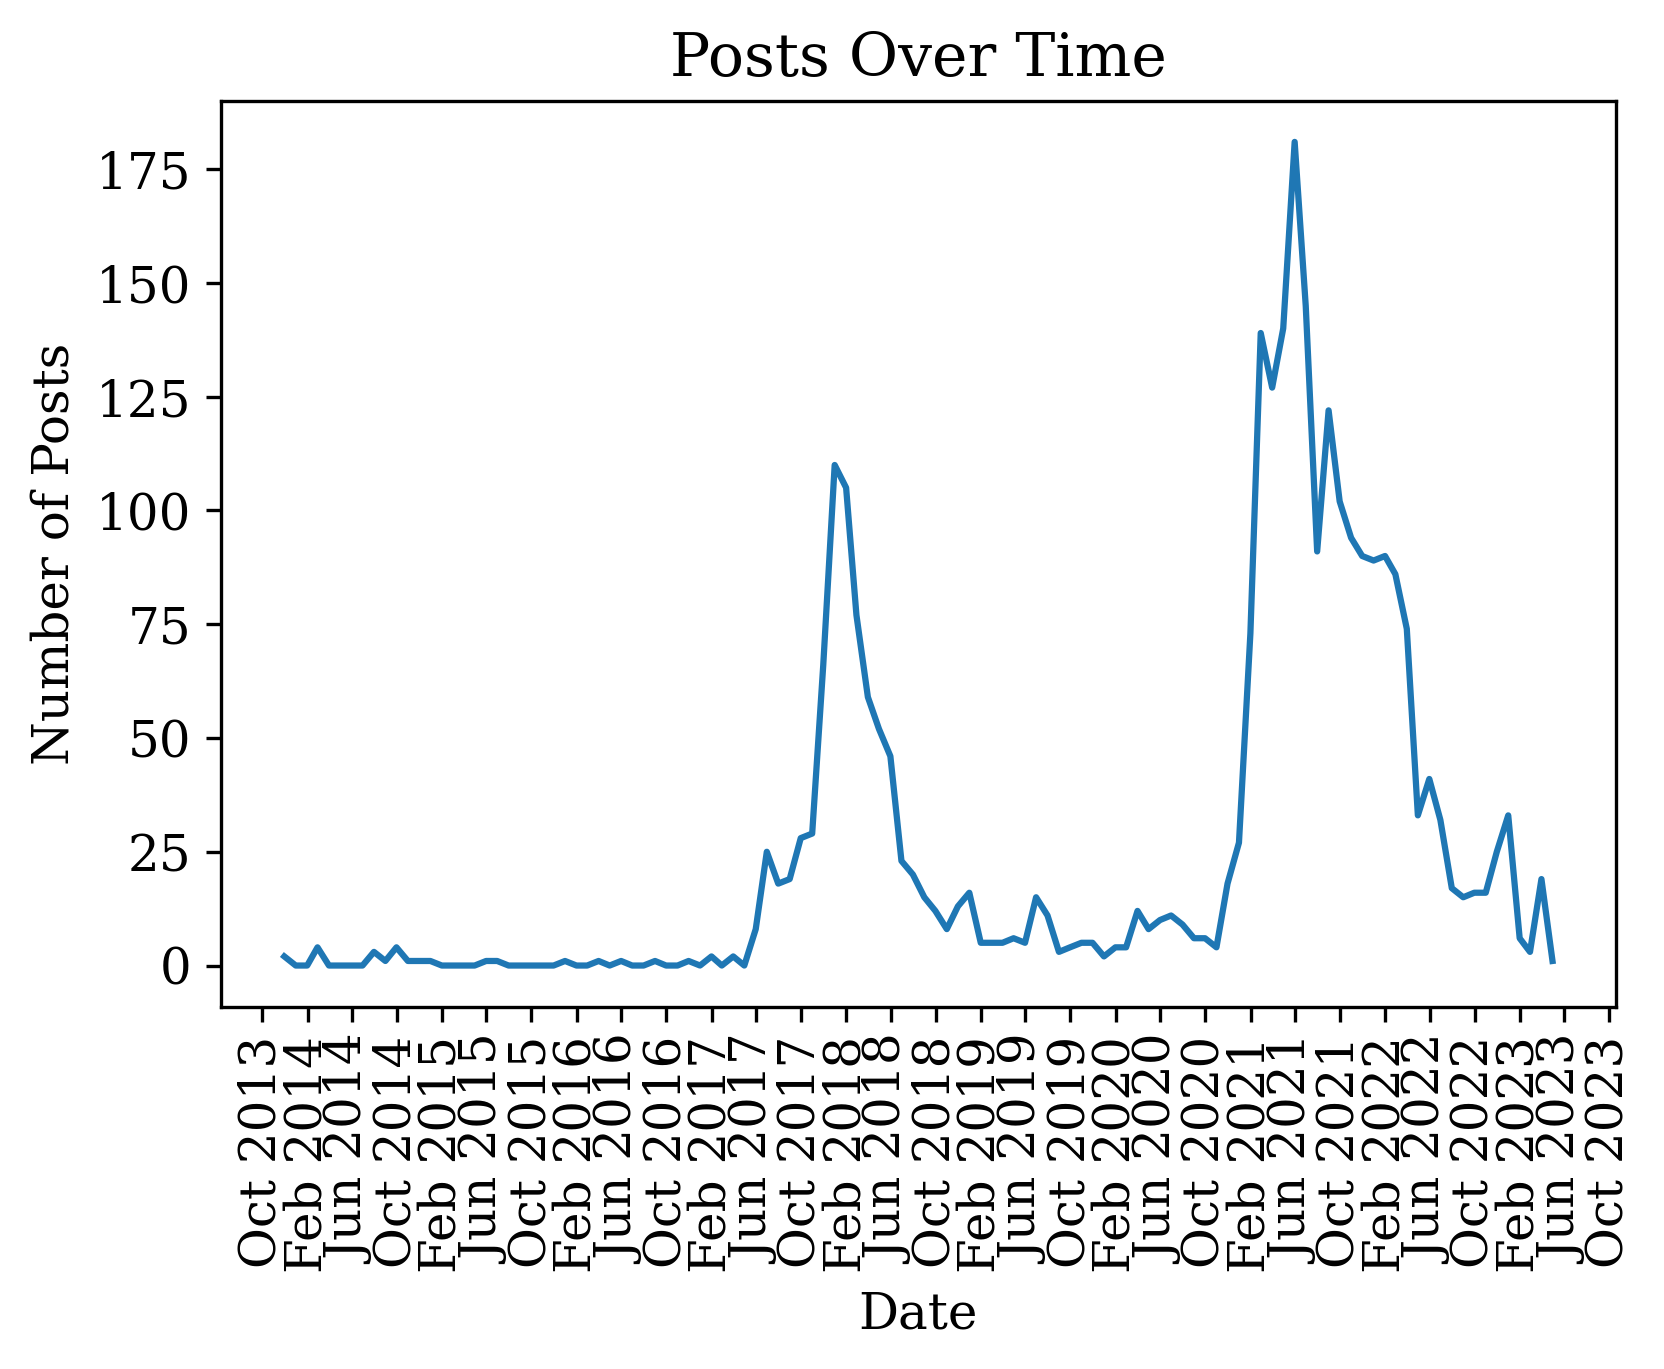
\includegraphics[scale=1]{img/A1/created_utc_timeseries.png}
\centering
\caption{Number of posts over time}
\label{fig:created_utc_timeseries}
\end{figure}

\begin{landscape}
We can compare Google Trends \parencite{web:GoogleTrends} searches to posts over time. By doing that, we see that post spikes matches with searches.
\begin{figure}[H]
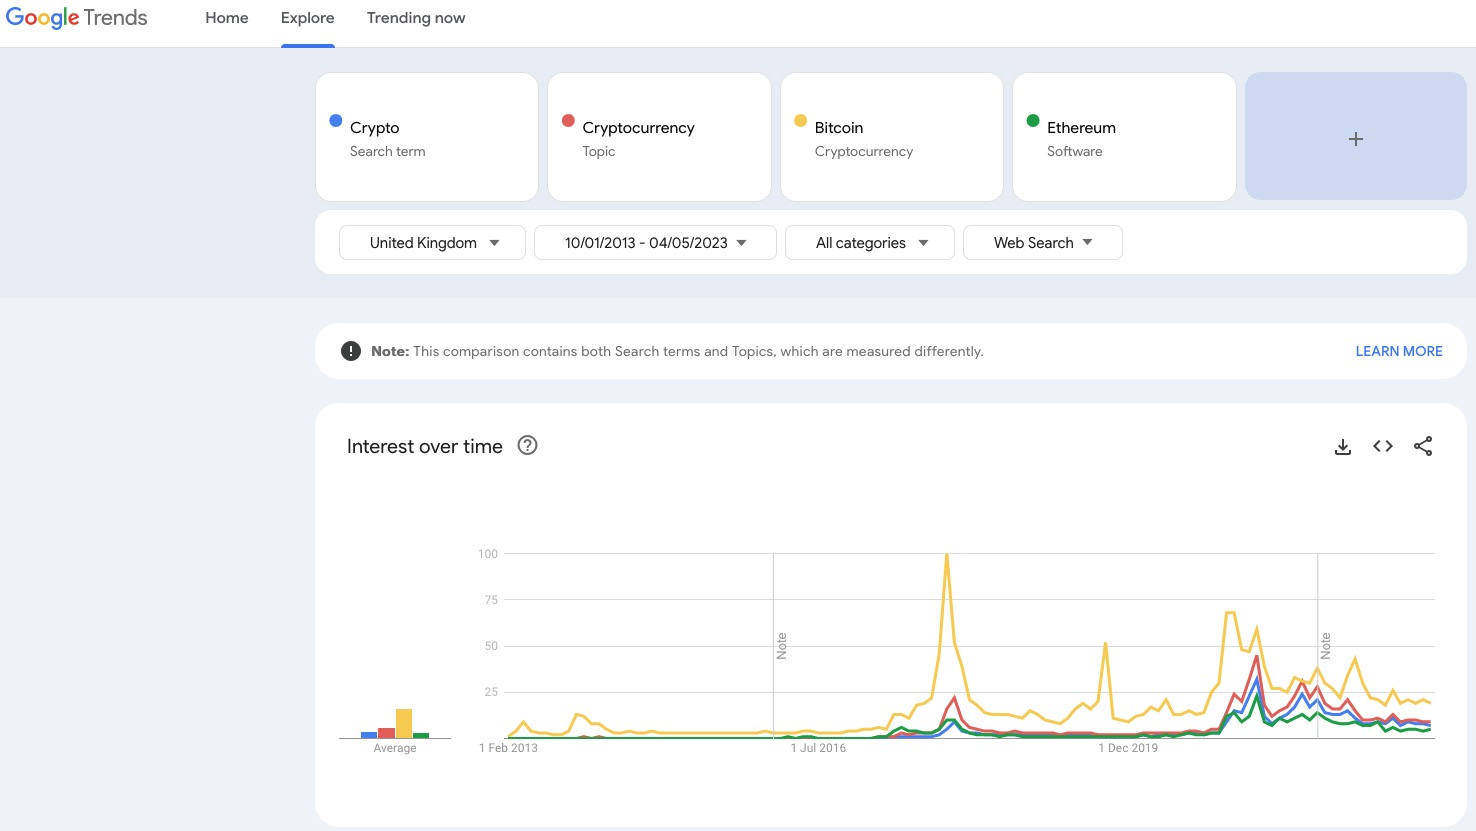
\includegraphics[scale=0.42]{img/A1/GoogleTrends.jpg}
\centering
\caption{Google Trends for crypto search}
\label{fig:GoogleTrends}
\end{figure}
\end{landscape}


If information is interesting, it drives a lot of attention. By this measure, does it mean that people will share (crosspost) this information more often due to its popularity?

The answer seems to be yes, since we can see that post with id 1066 has the highest number of crossposts and highest number  of duplicates as well. After that there seems to be a decline for number of duplicates is somewhat correlated to number of crossposts. But there are some outliers (eg post 2147) that showcases number of duplicates being lower. One of the reasons this can be is post moderation (even auto moderation) where duplicates are removed automatically.
\begin{figure}[H]
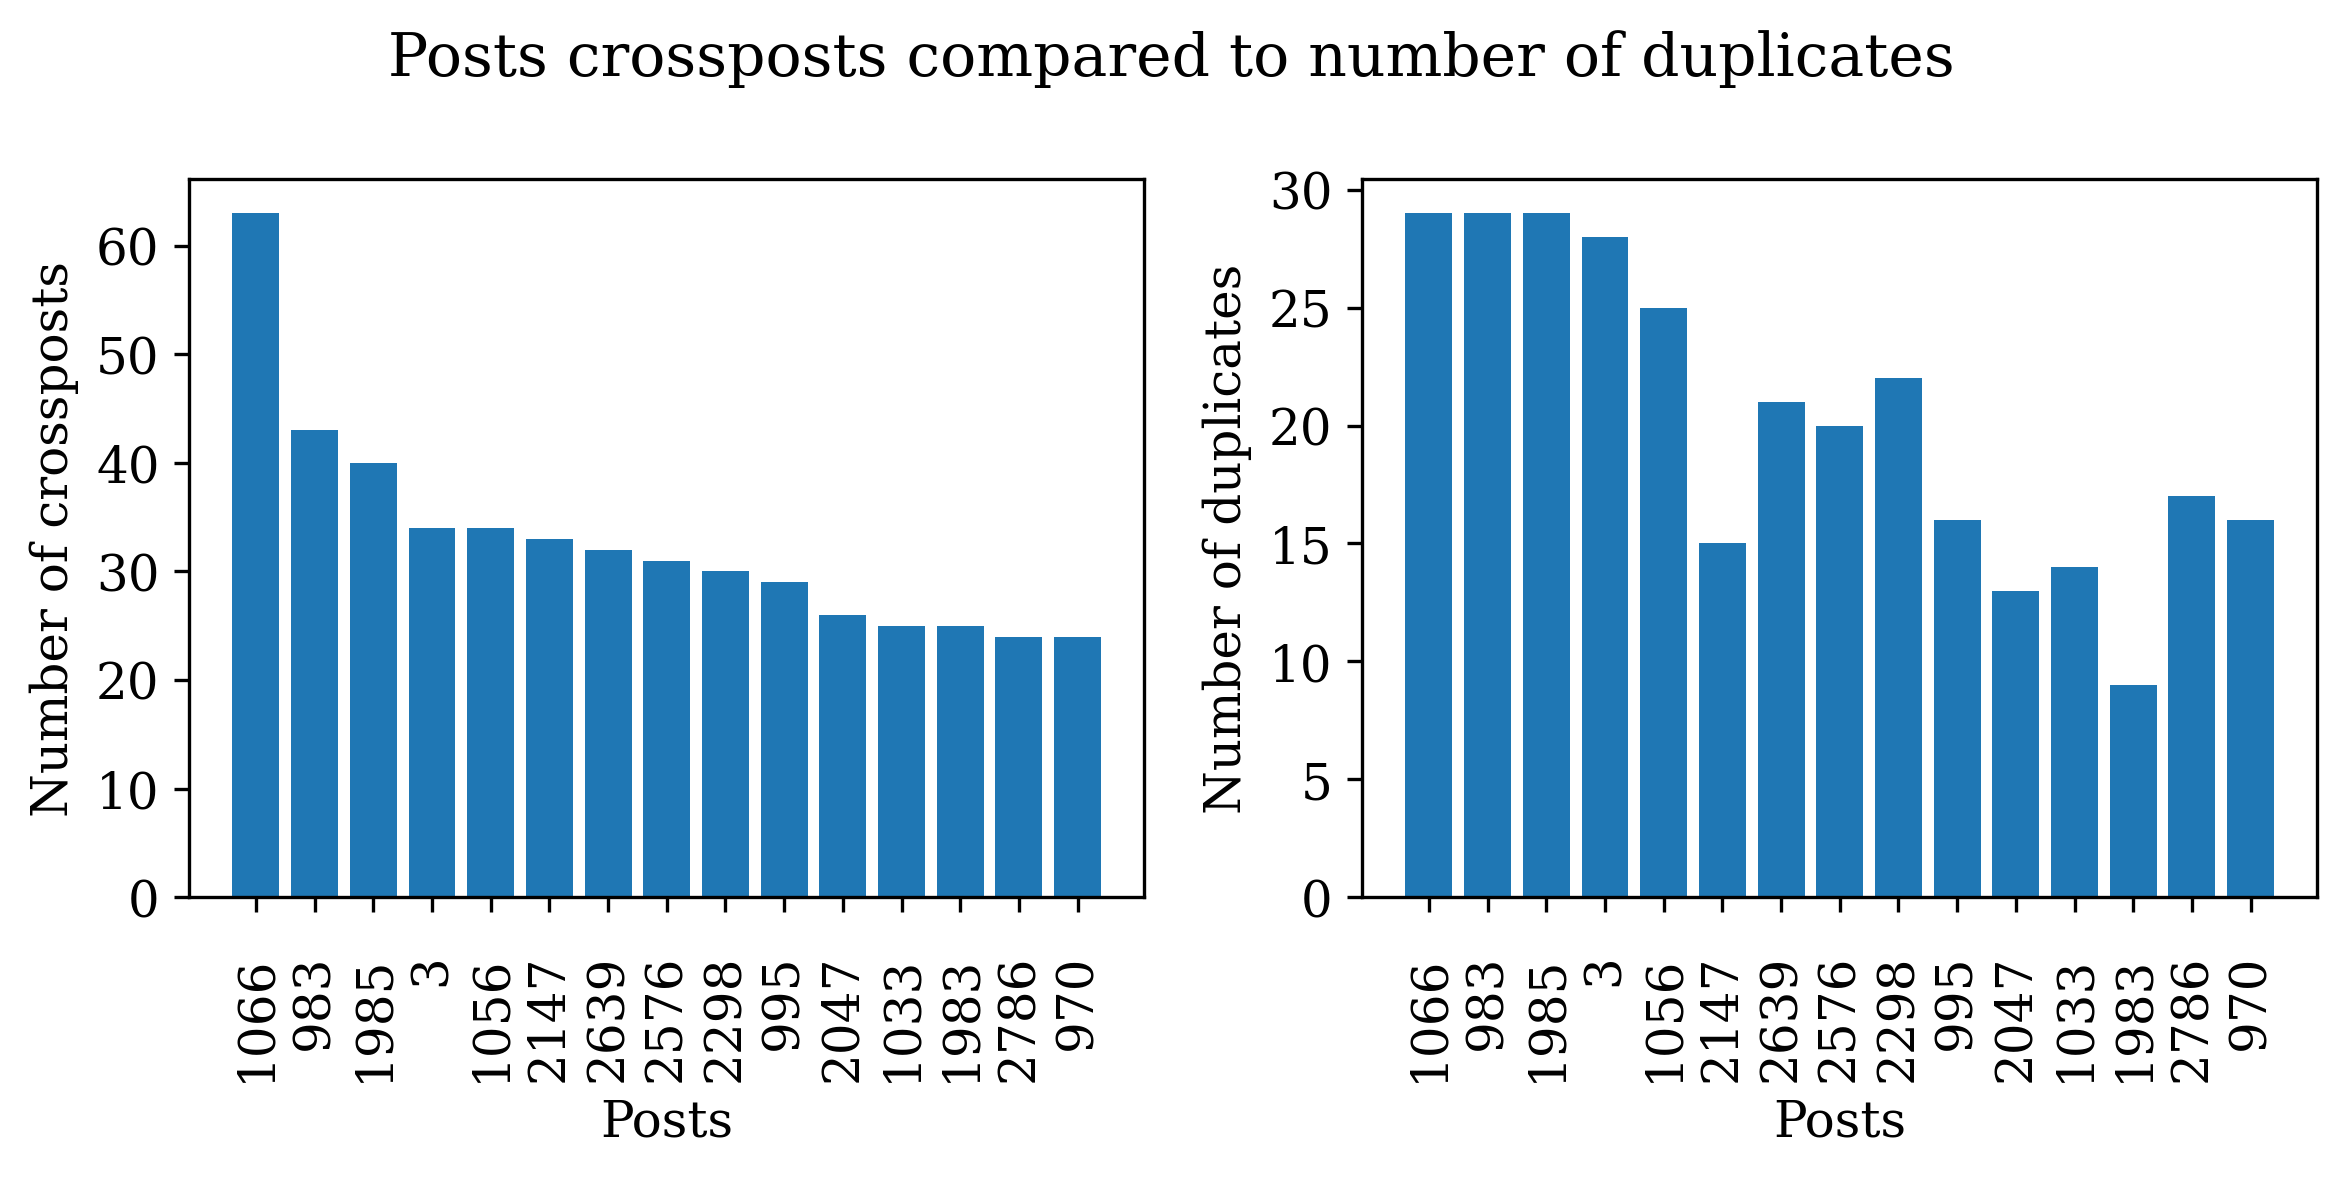
\includegraphics[scale=0.70]{img/A1/num_crossposts_double_histogram.png}
\centering
\caption{Crossposts and duplicates compared}
\label{fig:num_crossposts_double_histogram}
\end{figure}


\begin{figure}[H]
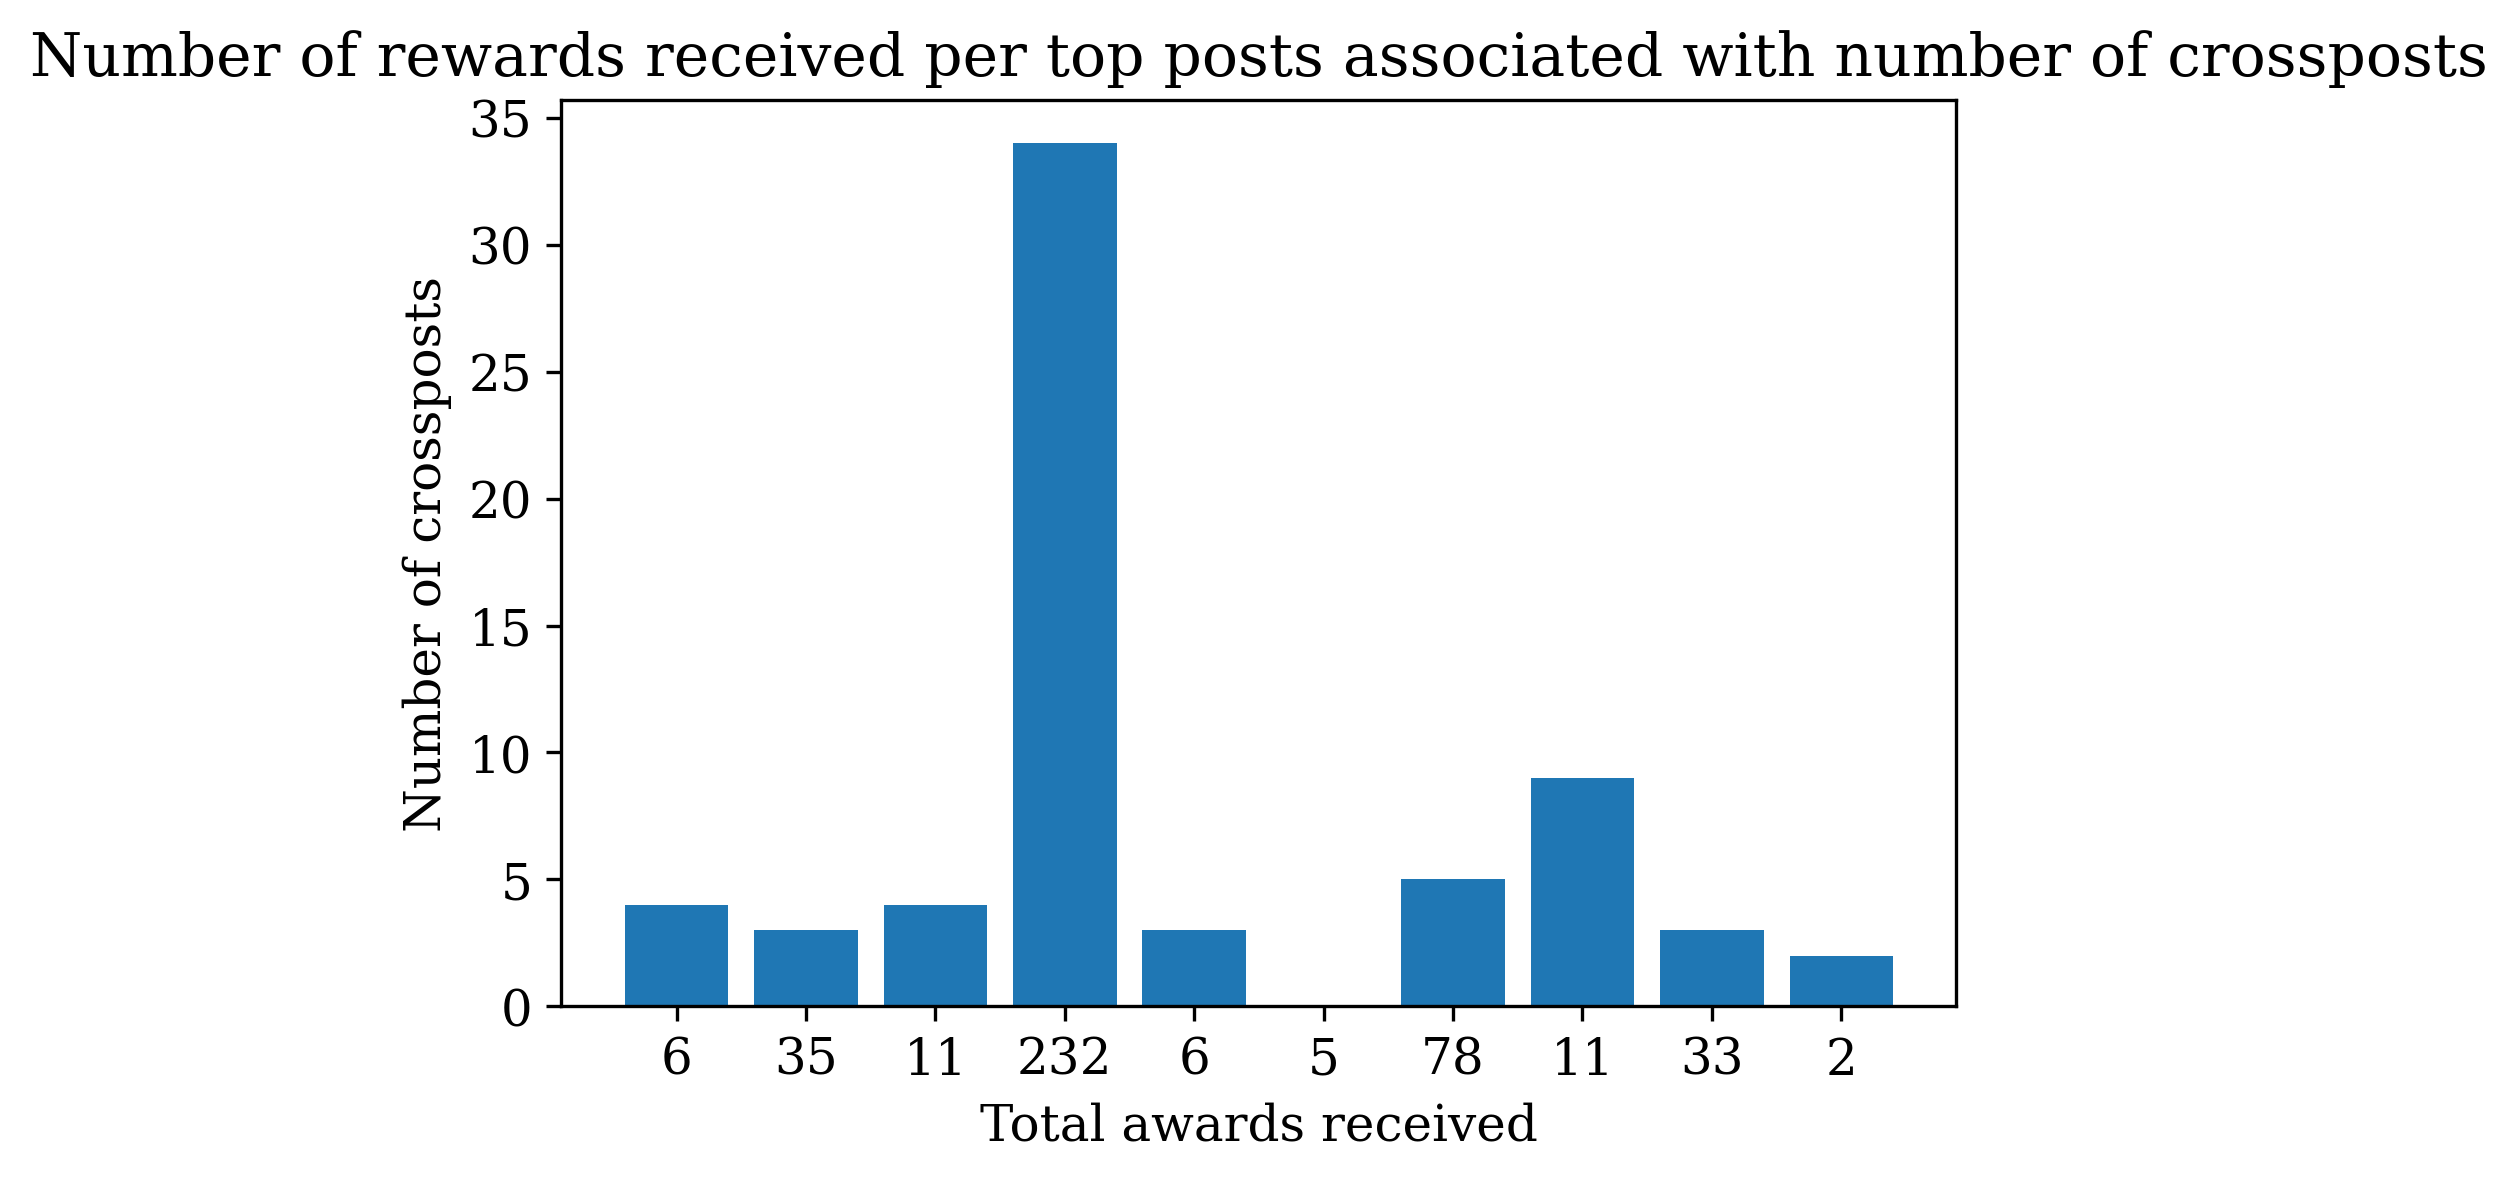
\includegraphics[scale=0.70]{img/A1/num_crossposts_plot.png}
\centering
\caption{Crossposts associated with rewards}
\label{fig:num_crossposts_plot}
\end{figure}


Assumption could be made that more comments post has more upvotes are there and more is it shared. 

It turns out that subreddits seem to isolate topics, which means that it doesn't matter how many upvotes or comments you will get, number of crossposts are not related to that. We can see the most upvoted post with 7741 upvotes is just a "regular post", while a 3rd largest post with 7444 upvotes has a lot of comments and not a lot crosspots. 4th largest post (7225) is opposite of 3rd one, it has a lot of crosspots but not a high amount of comments.
\begin{figure}[H]
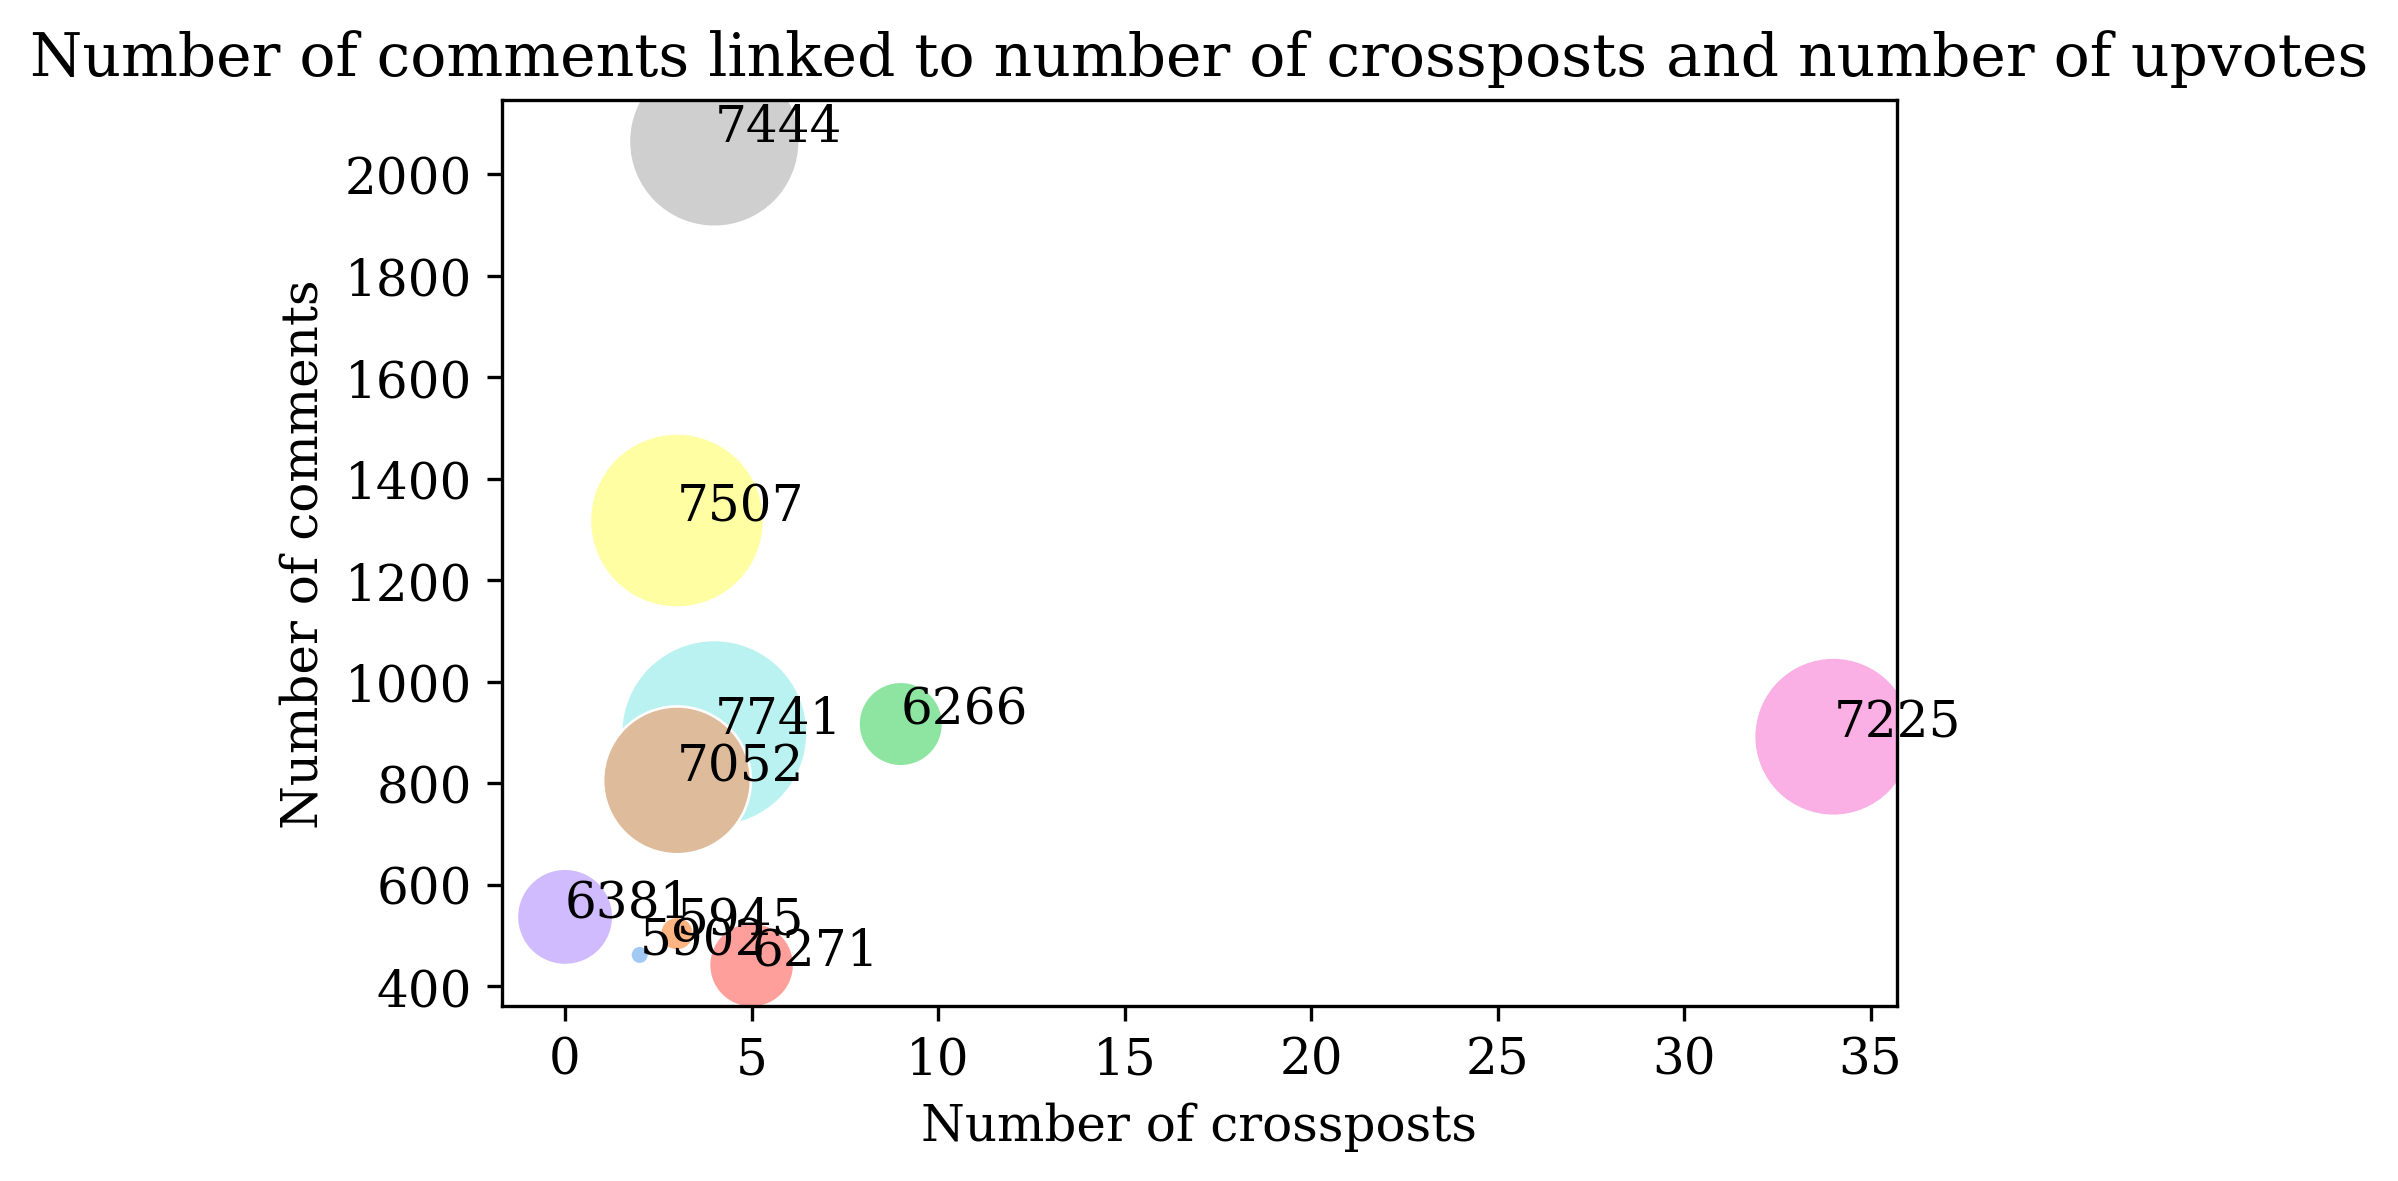
\includegraphics[scale=0.70]{img/A1/num_crossposts_scatterplot.png}
\centering
\caption{Number of comments correlated with with crosspots}
\label{fig:num_crossposts_scatterplot}
\end{figure}

Being active poster in the community will bring users some recognition. We can see that users with more posts, have higher number of upvotes.
\begin{figure}[H]
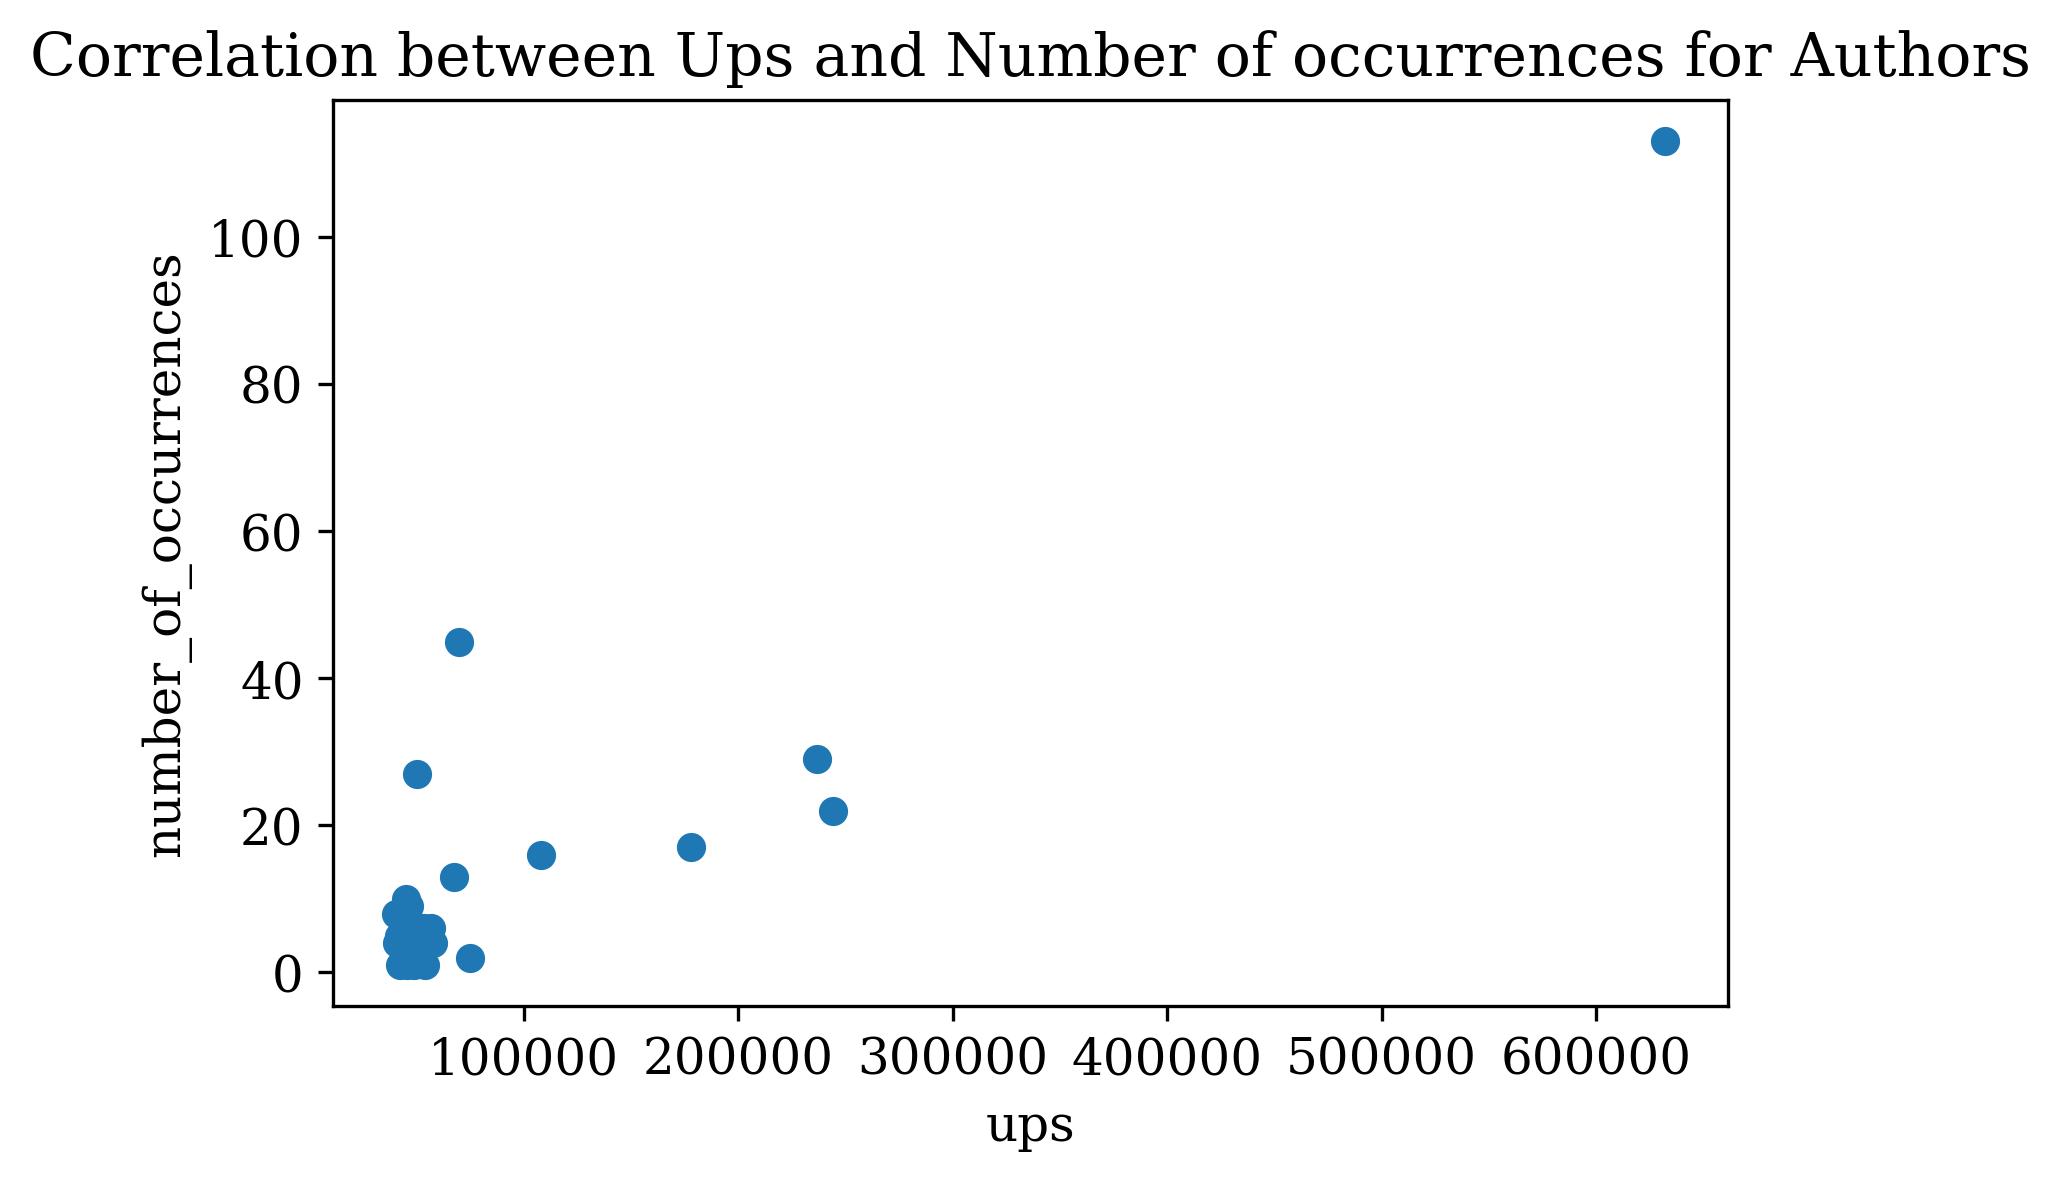
\includegraphics[scale=0.80]{img/A1/ups_scatterplot_simple.png}
\centering
\caption{Number of upvotes per user}
\label{fig:ups_scatterplot_simple}
\end{figure}

Post upvotes and awards are not correlated. If a post is more popular, it will not get more awards. 
\begin{figure}[H]
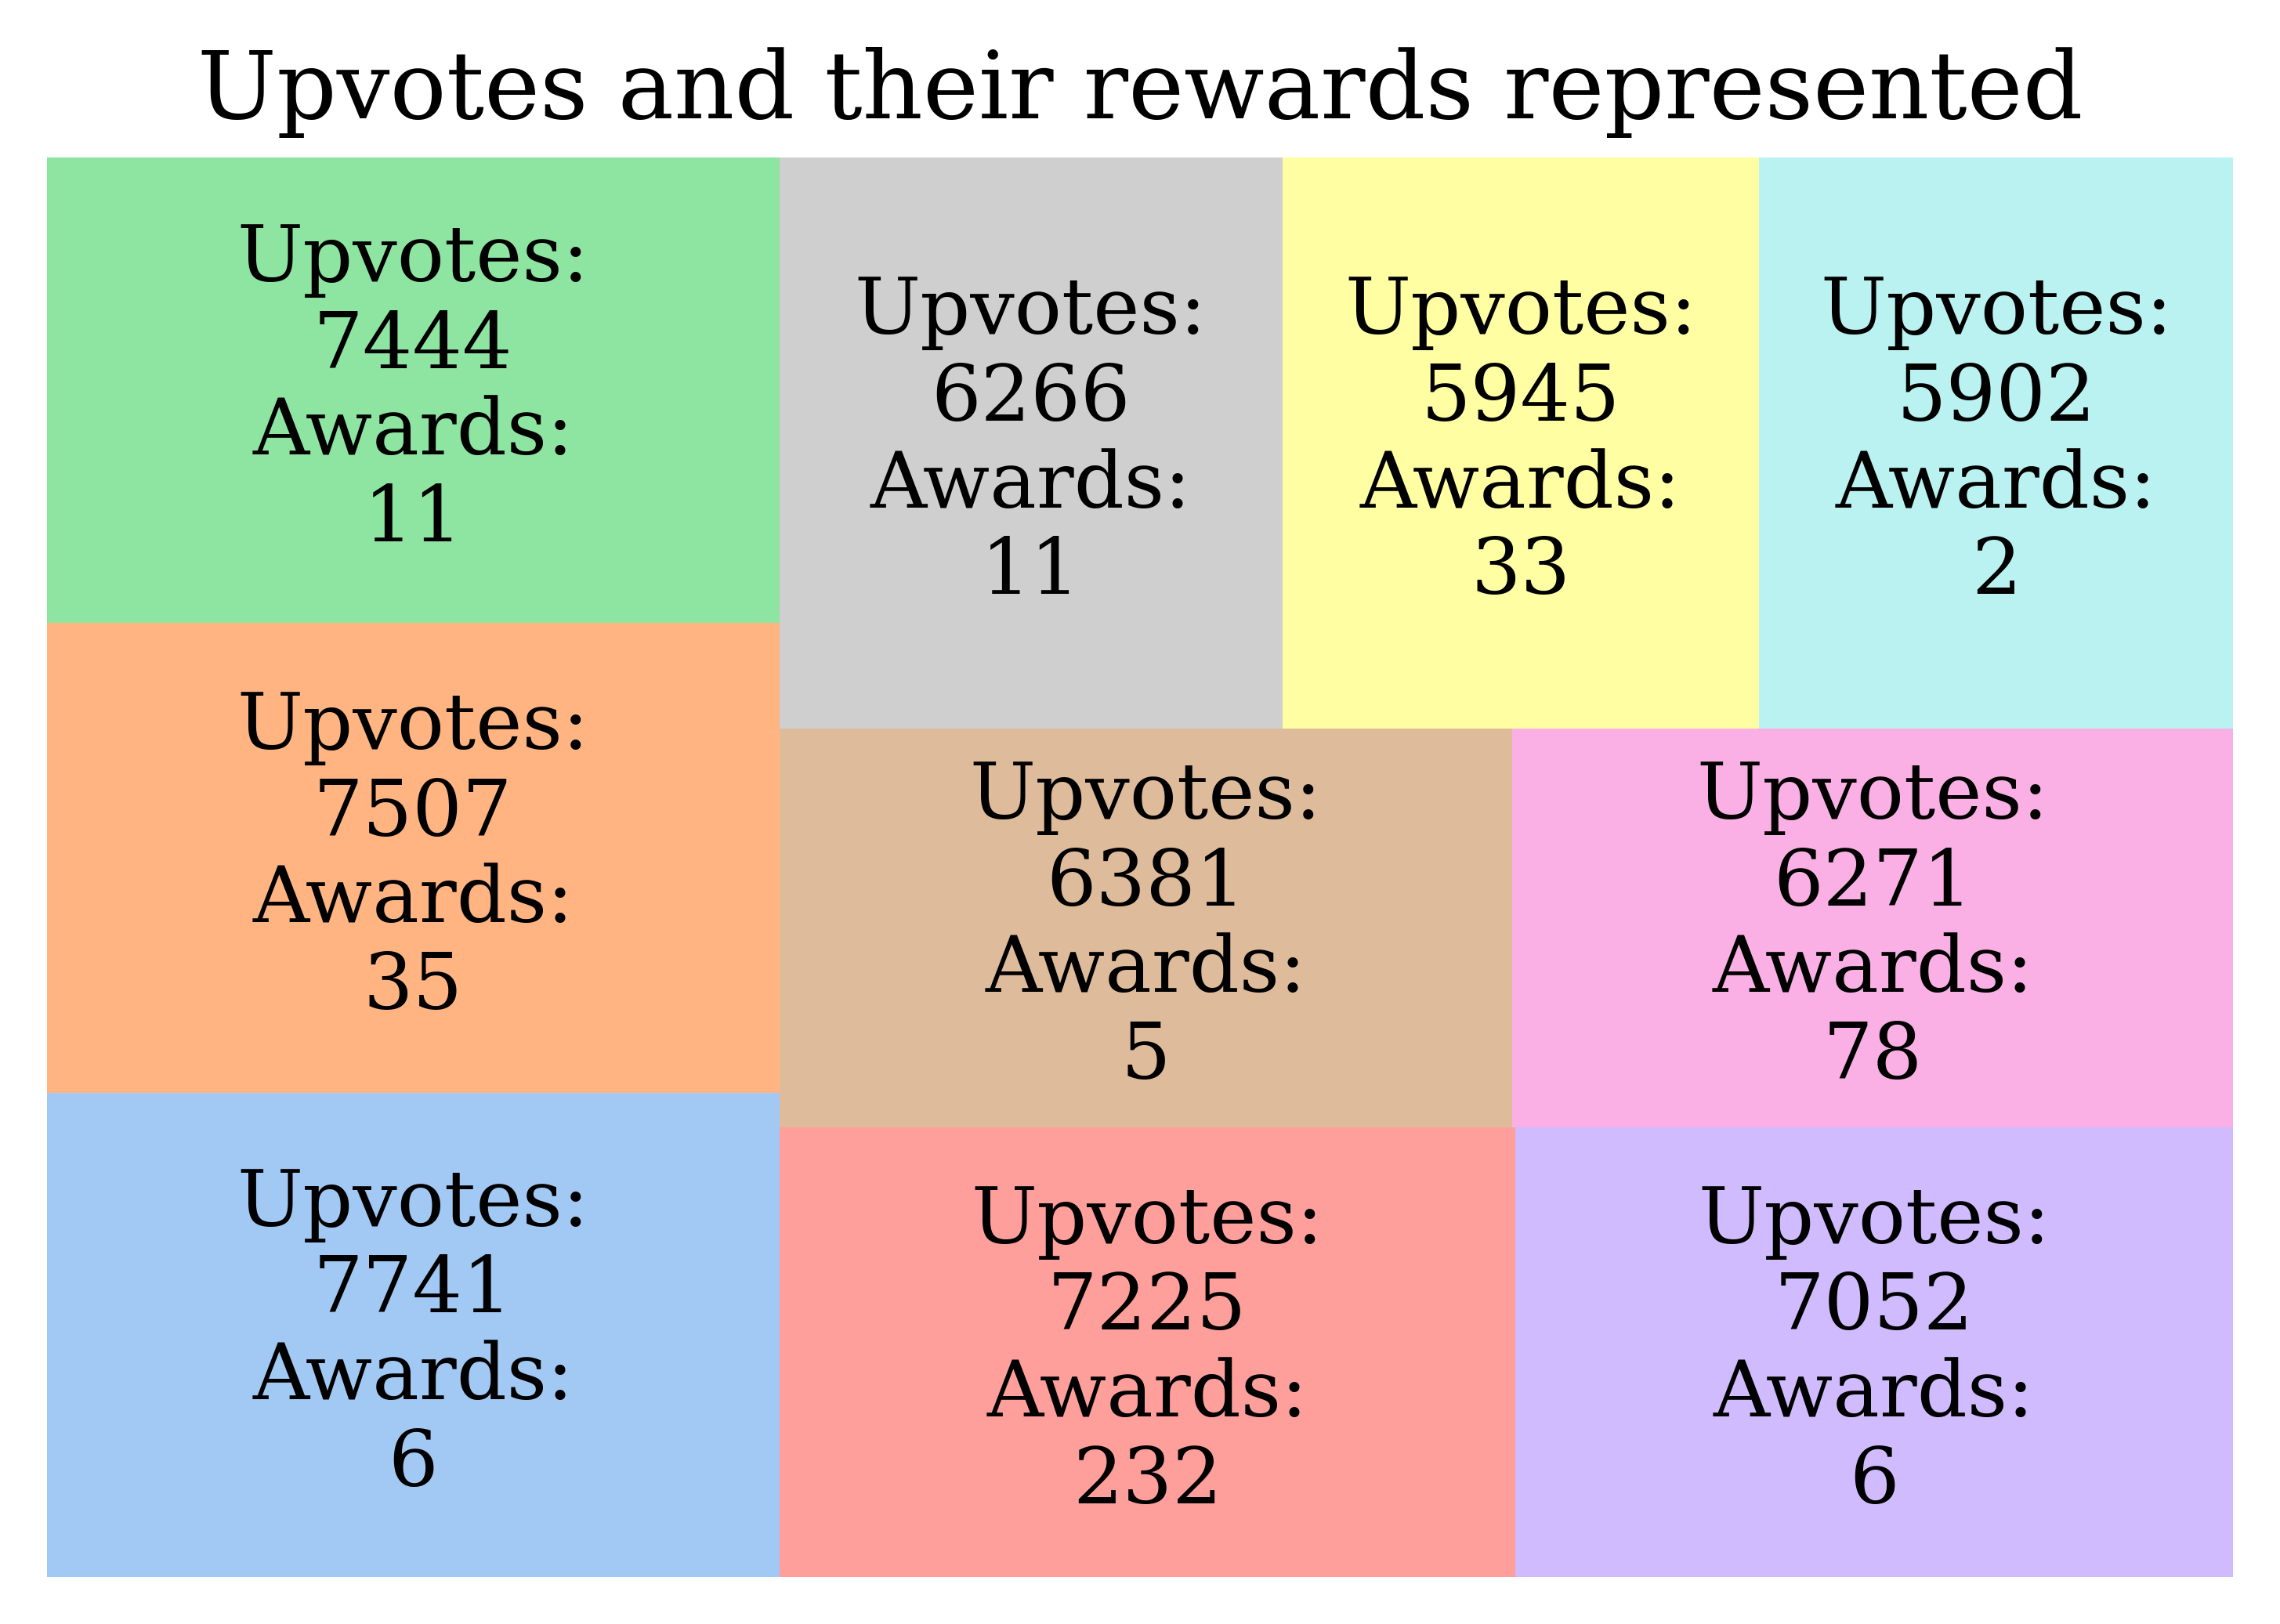
\includegraphics[scale=0.90]{img/A1/ups_treemap.png}
\centering
\caption{Top posts and their awards}
\label{fig:ups_treemap}
\end{figure}